
\begin{frame}{XAI: Enhancing Model Explainability}

    \textbf{Moving Towards Explainable AI for Sleep Staging}
    \vspace{0.5cm}
    
    \begin{itemize}
        \item \textbf{Why Explainability?}  
              - Medical experts need transparency in AI decisions for trust and adoption.  
              - Understanding how features influence sleep stage transitions is crucial.
              
        \item \textbf{Current Achievements:}  
              - \textcolor{blue}{\textbf{GCN:}} Captures spatial relationships between EEG channels.  
              - \textcolor{blue}{\textbf{Transformer:}} Captures temporal dependencies in sleep data.  
              - Achieved state-of-the-art accuracy using both approaches.
              
        \item \textbf{Next Steps:}  
              - Implement AI-driven methods to highlight critical sleep stage transition points.  
              - Develop feature attribution methods to understand the importance of each signal.  
              - Improve model interpretability to align with clinical expectations.
    \end{itemize}

\end{frame}


\begin{frame}{XAI: Sleep Stage Focus — N1 and N2}
	\textbf{Visualizing Model Attention on Light Sleep Stages}
	\vspace{0.3cm}
	
	\begin{itemize}
		\item N1 and N2 stages show low-frequency waveforms and spindles.
		\item The model highlights relevant signal segments using XAI techniques.
	\end{itemize}
	
	\begin{figure}
		\centering
		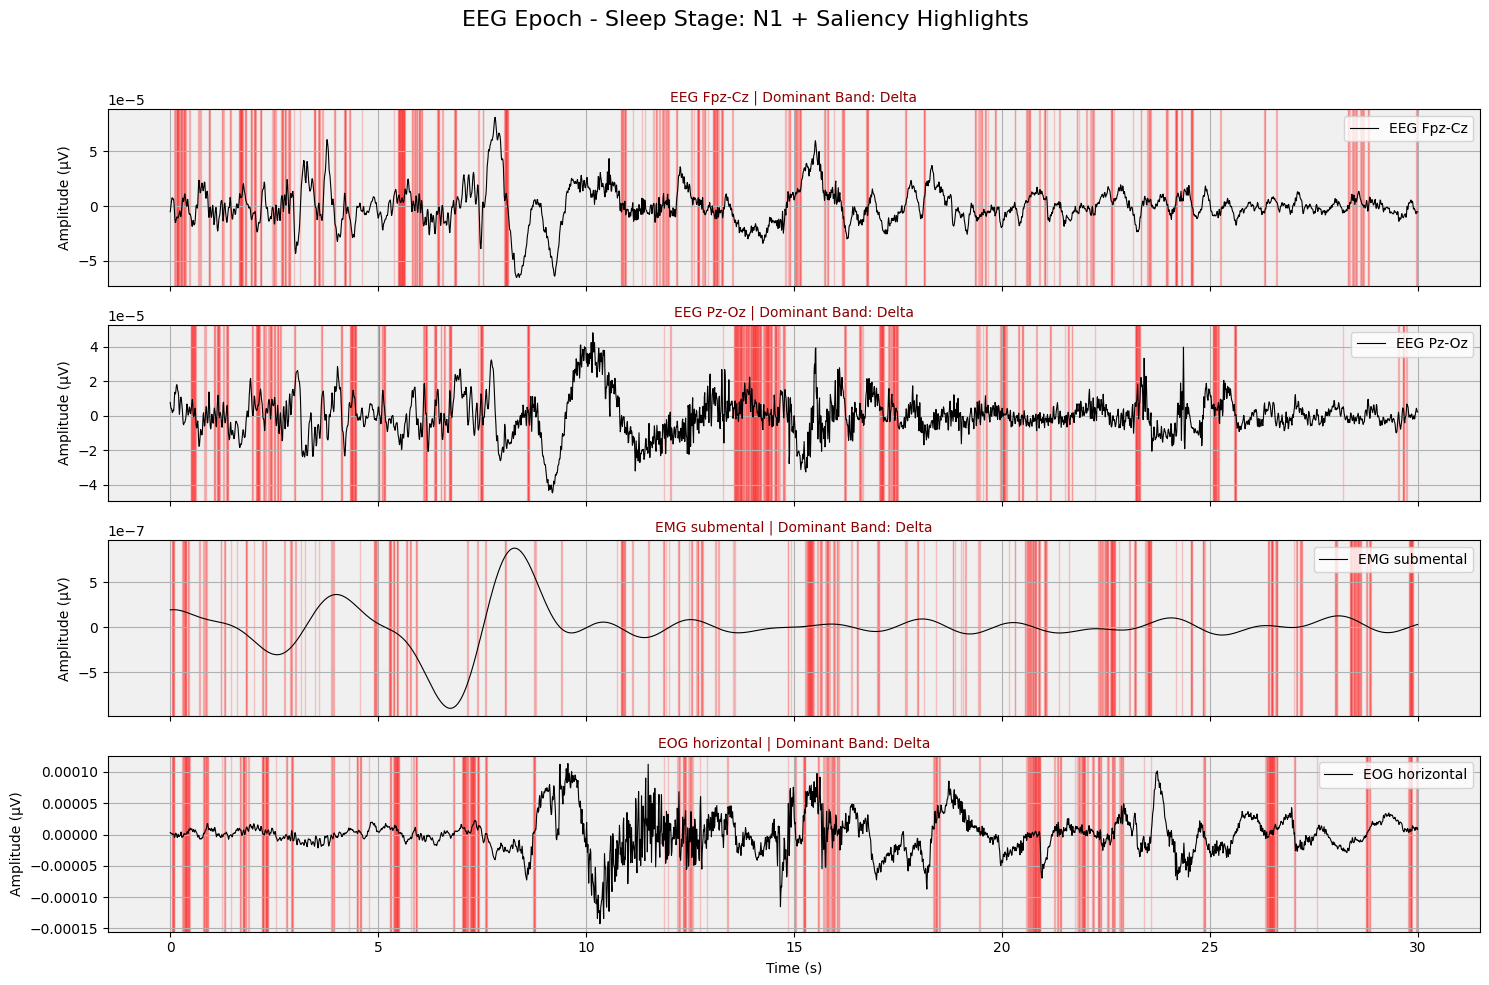
\includegraphics[width=0.45\linewidth]{images/paper_3/stagen1.png}
		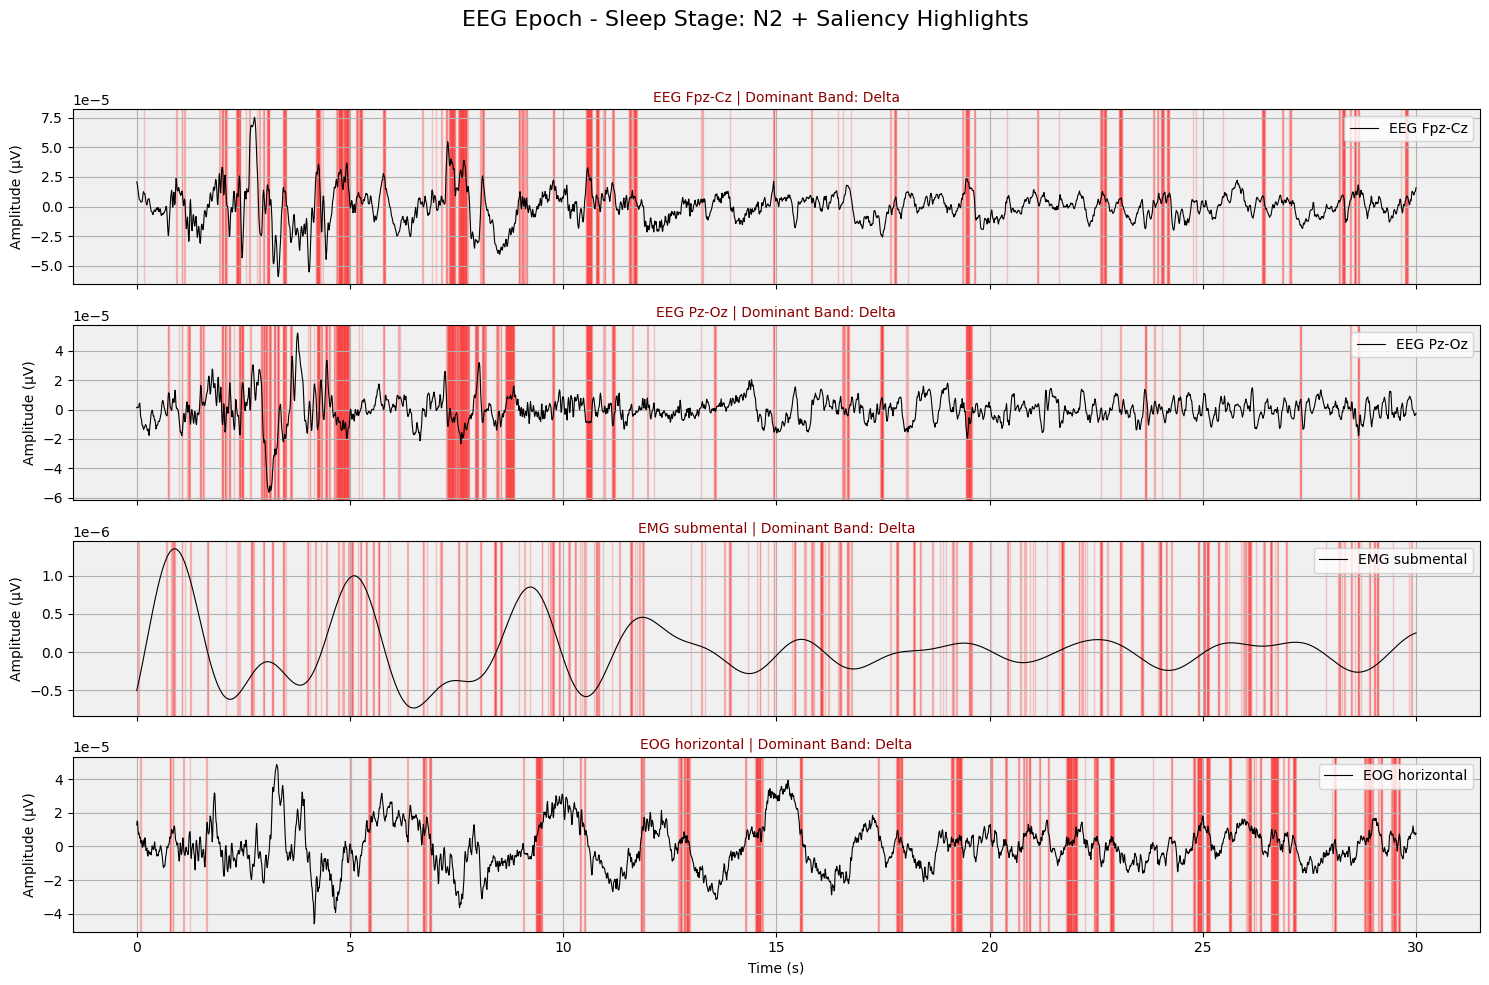
\includegraphics[width=0.45\linewidth]{images/paper_3/stagen2.png}
		\caption{XAI Highlights for Stage N1 (left) and N2 (right)}
	\end{figure}
\end{frame}

\begin{frame}{XAI: Sleep Stage Focus — N3 and REM}
	\textbf{Explaining Deep Sleep and REM Predictions}
	\vspace{0.3cm}
	
	\begin{itemize}
		\item Stage N3 shows slow-wave activity; REM features resemble wake but with eye movement signals.
		\item Model interpretability reveals key distinguishing signal patterns.
	\end{itemize}
	
	\begin{figure}
		\centering
		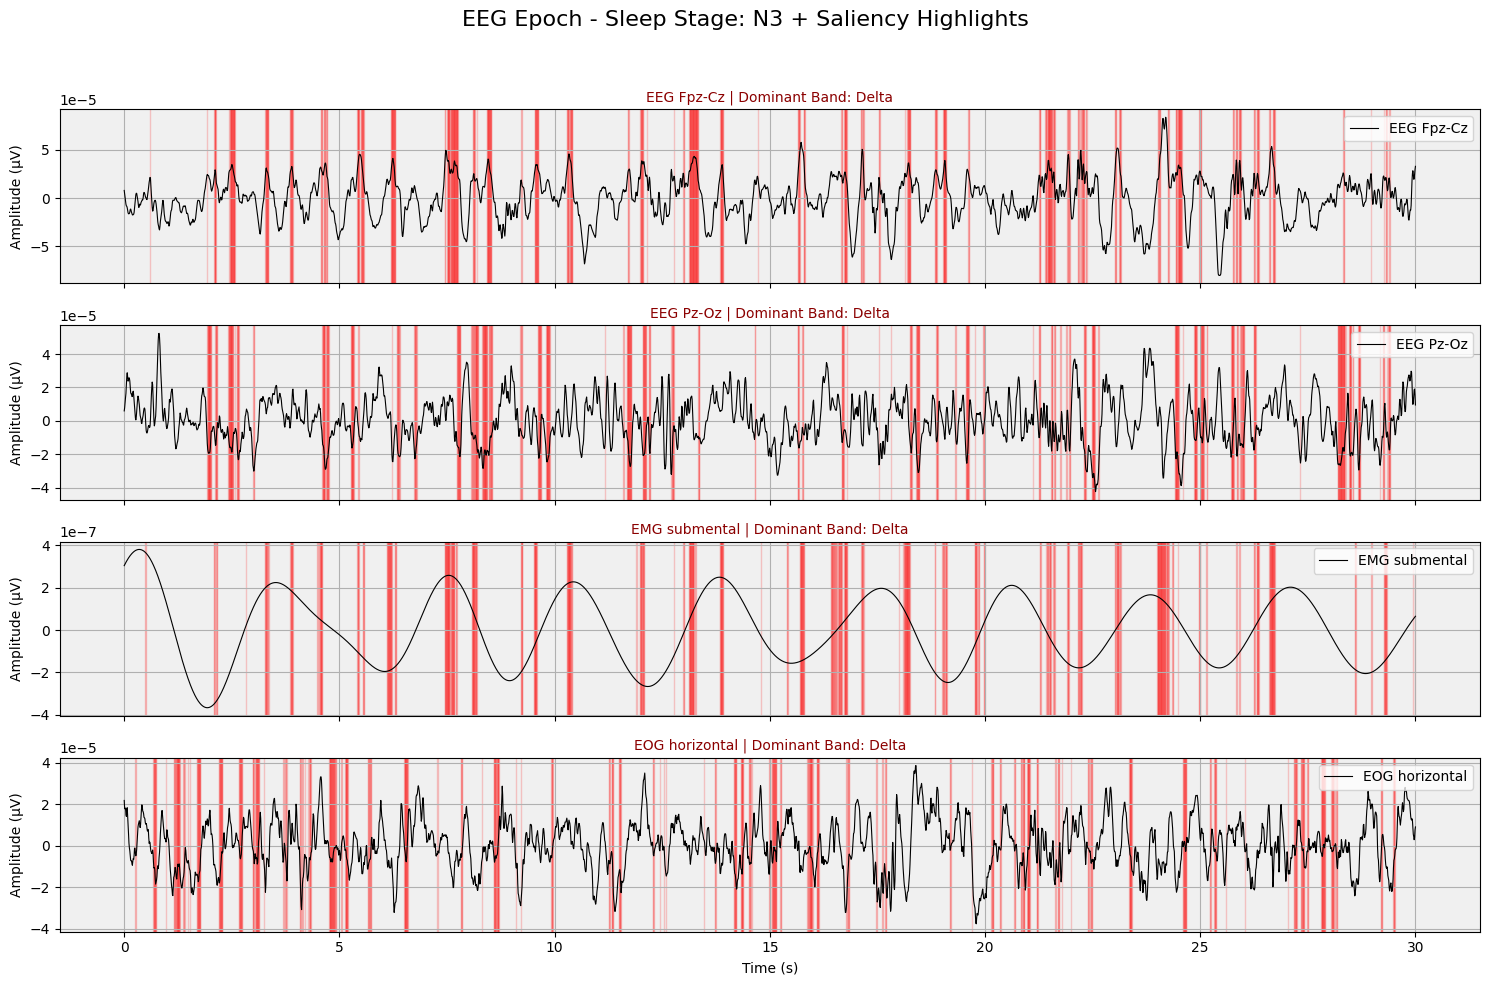
\includegraphics[width=0.45\linewidth]{images/paper_3/stagen3.png}
		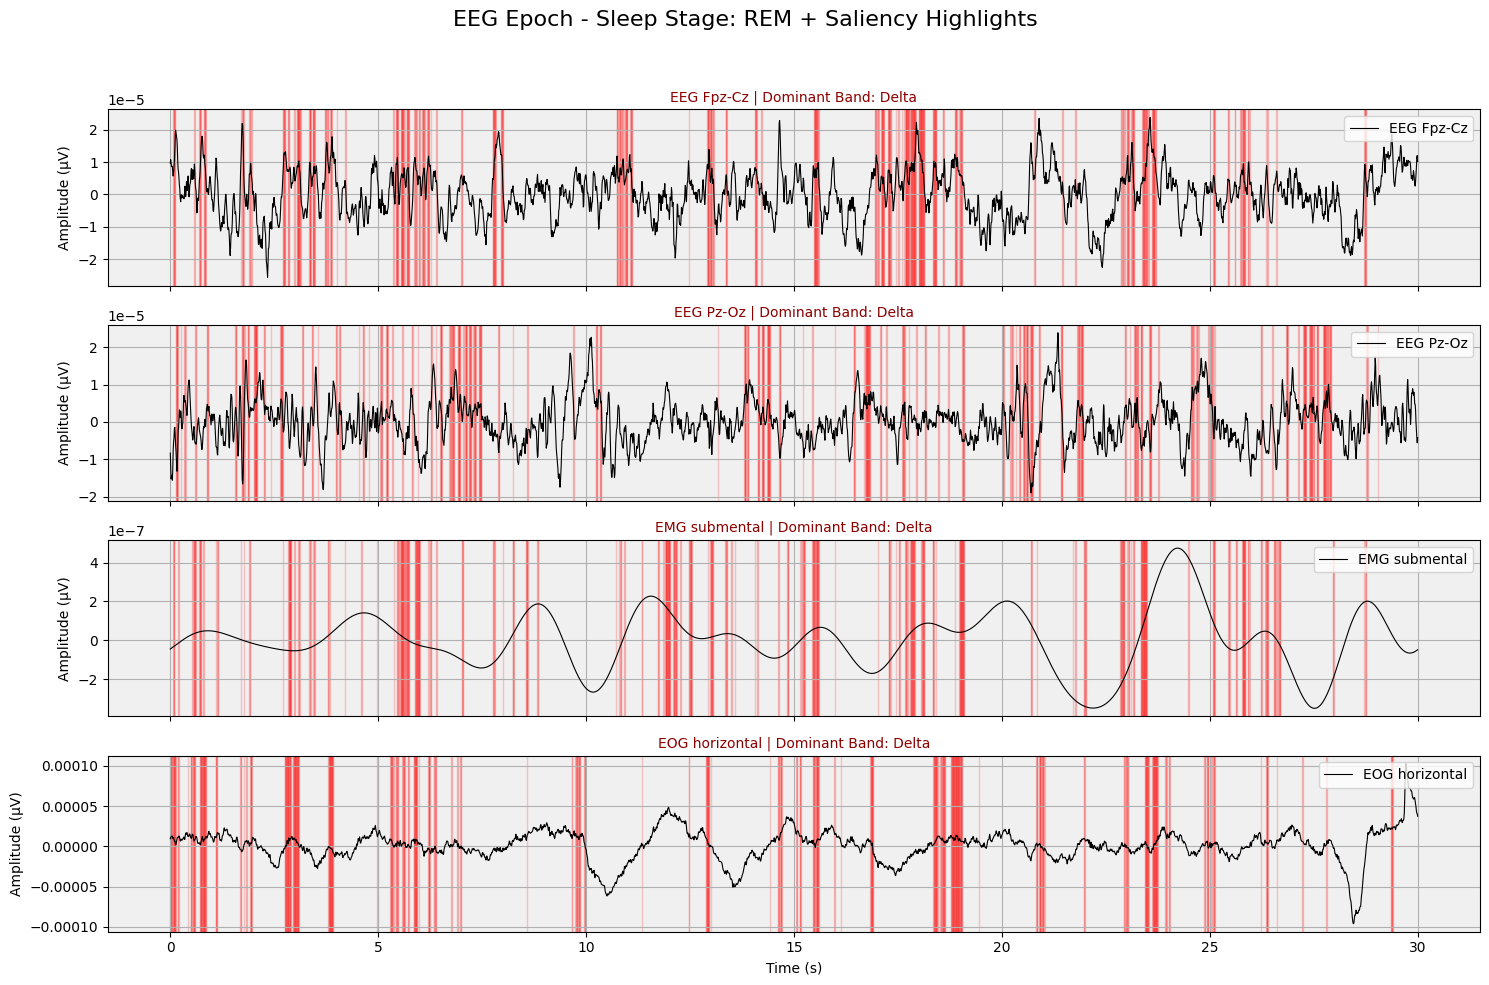
\includegraphics[width=0.45\linewidth]{images/paper_3/stagerem.png}
		\caption{XAI Highlights for Stage N3 (left) and REM (right)}
	\end{figure}
\end{frame}

\begin{frame}{XAI: Wakefulness and Global Insight}
	\textbf{Model Explanation for Wake Stage and Summary Map}
	\vspace{0.3cm}
	
	\begin{itemize}
		\item Wake stage shows fast, high-frequency signals.
		\item The full-view XAI map summarizes attention across all classes.
	\end{itemize}
	
	\begin{figure}
		\centering
		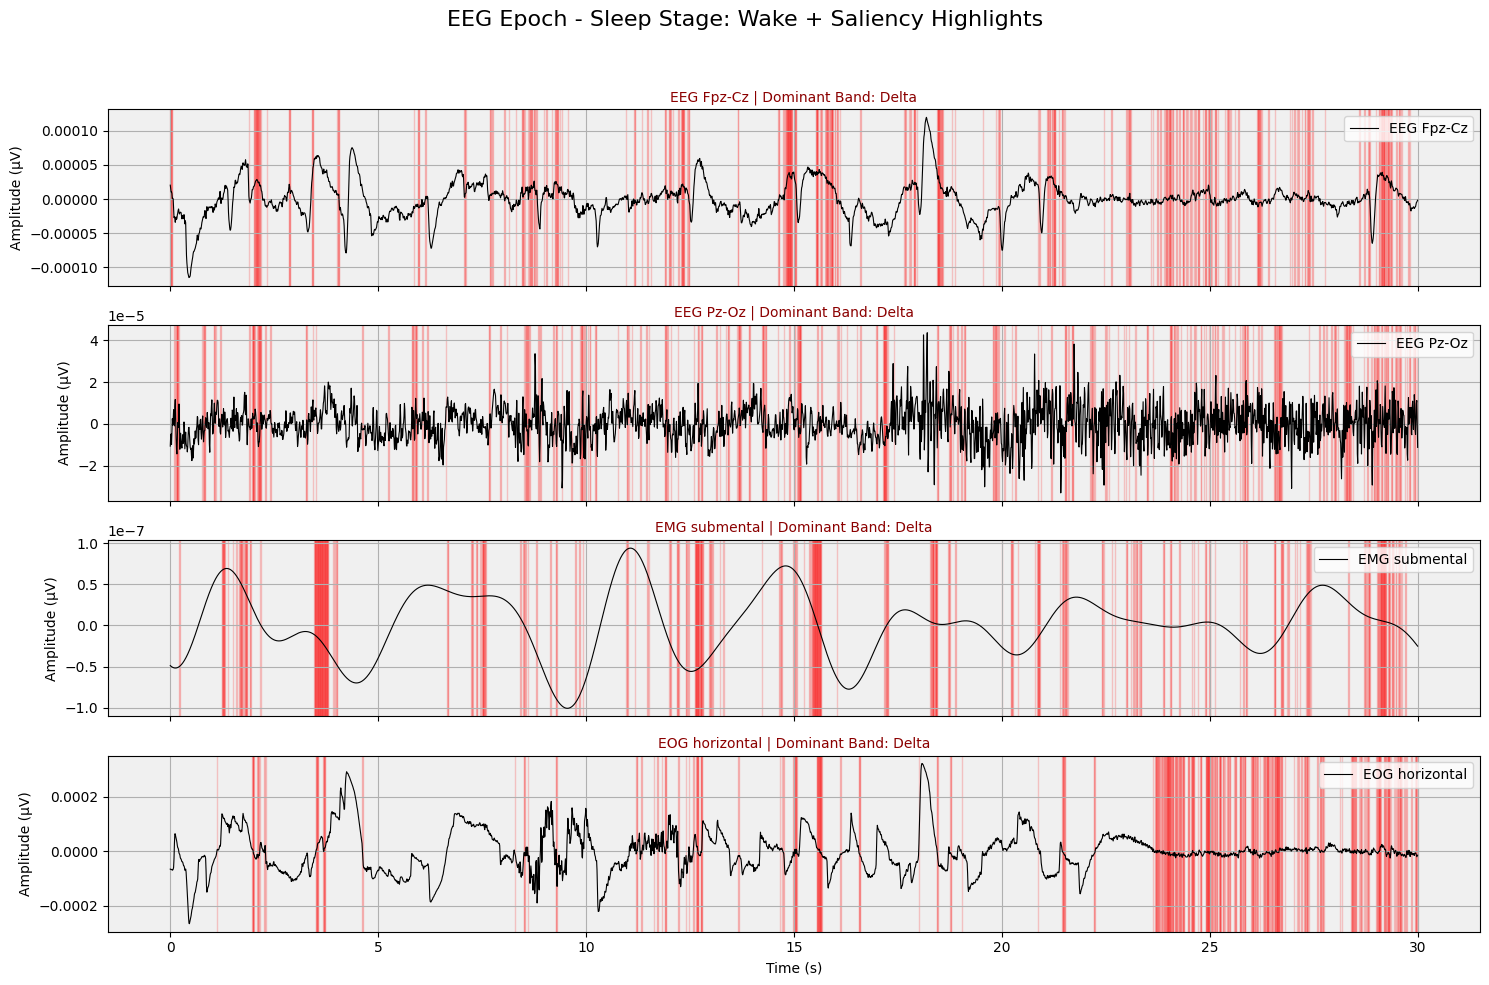
\includegraphics[width=0.45\linewidth]{images/paper_3/stagewake.png}
		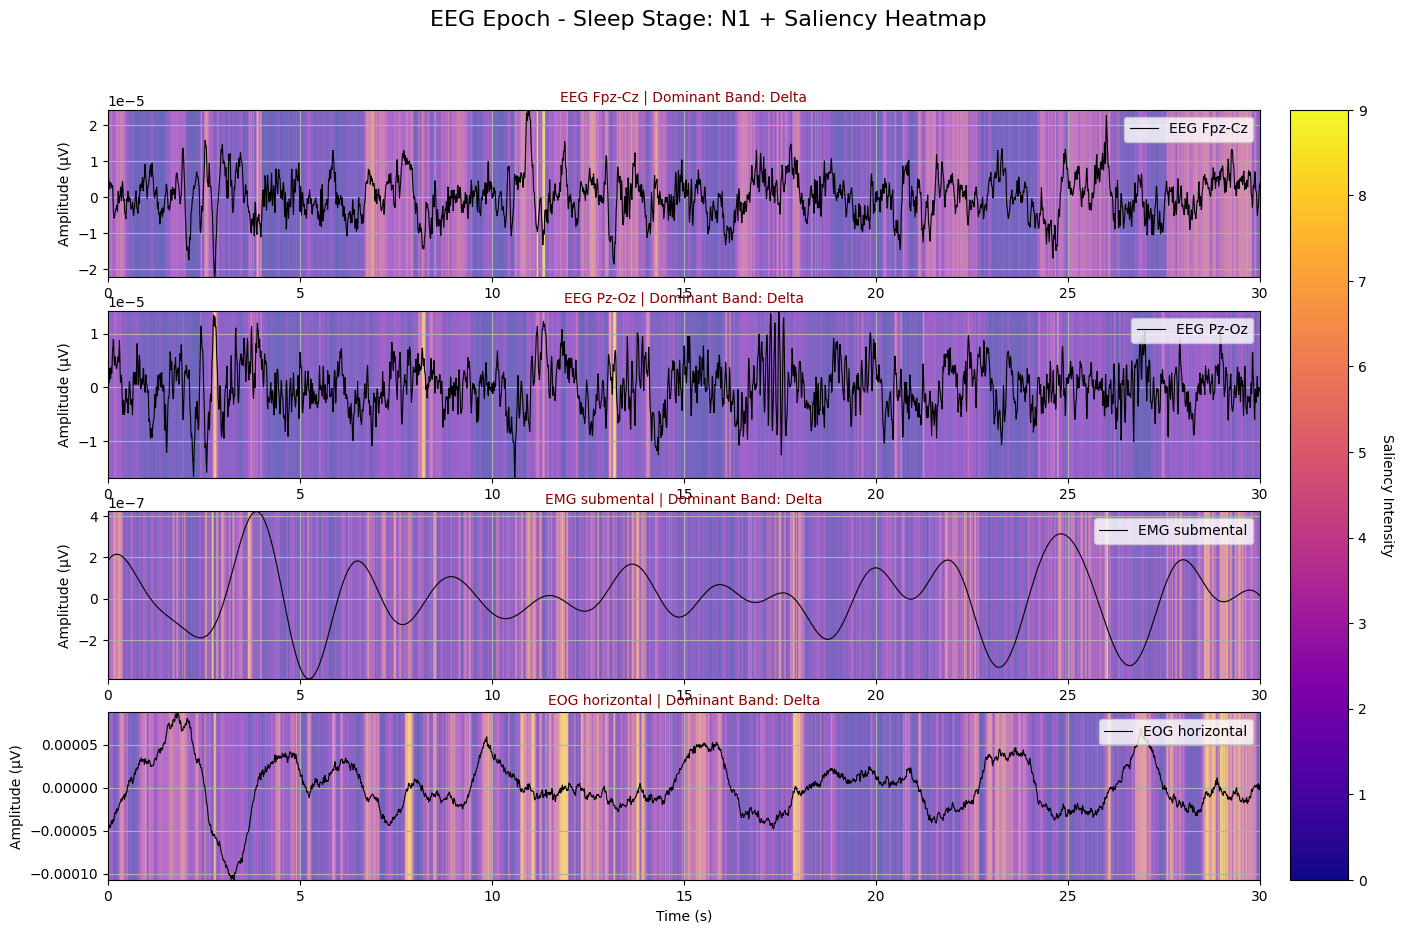
\includegraphics[width=0.45\linewidth]{images/paper_3/XAI4.png}
		\caption{Wake Stage (left) and Overall XAI Map (right)}
	\end{figure}
\end{frame}


 



\begin{frame}{Future Plan: AI for Sleep Science and Clinical Use}

    \begin{columns}
        % Left Column: Explanation
        \column{0.55\textwidth}
        
        \textbf{Bridging AI and Healthcare}
        \begin{itemize}
            \item \textbf{Feature Importance:} Identify which EEG channels contribute most to predictions.
            \item \textbf{Clinical Relevance:} Provide insights that can be validated by sleep specialists.
            \item \textbf{Graph + Transformer Insights:}
            \begin{itemize}
                \item \textcolor{blue}{\textbf{GCN:}} Capturing inter-channel spatial dependencies.
                \item \textcolor{blue}{\textbf{Transformer:}} Learning sequential patterns across sleep cycles.
            \end{itemize}

                    \end{itemize}

        % Right Column: Block Diagram
       % Right Column: Block Diagram
\column{0.45\textwidth}
\centering
\begin{tikzpicture}
    % Nodes
    \node[draw, text width=3cm, align=center, fill=blue!20, rounded corners] 
        (gcn) {\footnotesize Graph Convolution (GCN) \\ \tiny Captures Spatial Relations};
        
    \node[draw, text width=3cm, align=center, fill=blue!40, rounded corners, below=0.6cm of gcn] 
        (transformer) {\footnotesize Transformer \\ \tiny Captures Temporal Patterns};
        
    \node[draw, text width=3cm, align=center, fill=purple!40, rounded corners, below=0.6cm of transformer] 
        (explainable) {\footnotesize Explainable AI \\ \tiny Sleep Stages \& Feature Analysis};
        
    \node[draw, text width=3cm, align=center, fill=green!40, rounded corners, below=0.6cm of explainable] 
        (medical) {\footnotesize Medical Integration \\ \tiny AI-Assisted Diagnosis};

    % Arrows
    \draw[->, thick] (gcn) -- (transformer);
    \draw[->, thick] (transformer) -- (explainable);
    \draw[->, thick] (explainable) -- (medical);
\end{tikzpicture}

    \end{columns}

\end{frame}

\begin{frame}{Conclusion}
	\begin{block}{}
		Our proposed SleepGCN-Transformer model achieves \textbf{93.12\% training accuracy} and \textbf{93.04\% validation accuracy}, demonstrating its effectiveness in sleep stage classification. The integration of \textbf{Graph Convolution Networks (GCN)} captures spatial dependencies across EEG, EOG, and EMG channels, while the \textbf{Transformer} extracts temporal patterns. The use of \textbf{Focal Loss} enhances class balancing, improving performance on underrepresented sleep stages. Feature importance analysis highlights \textbf{EMG and EEG Pz-Oz} as key predictors. This robust approach lays the foundation for future work in \textbf{Explainable AI}, enabling medical professionals to interpret AI-driven sleep diagnostics effectively.
	\end{block}
\end{frame}

\begin{frame}{Publications}
	\begin{block}{}
		\textbf{1. Automated Sleep Staging System with EEG Signal using Machine Learning Techniques} \\
		Santosh Kumar Satapathy, Tanmay Rathod, Nibedita Das, Rajesh Kumar Mohapatra, Suren Sahu, Jaynil Joshi, 2025 IEEE International Conference on Interdisciplinary Approaches in Technology and Management for Social Innovation (IATMSI). \url{https://ieeexplore.ieee.org/document/10985276} \\
		
		\textbf{2. Automated Sleep Staging System Using EEG Signal Feature-Based Classification by Machine Learning Techniques} \\
		Tanmay Rathod, Santosh Kumar Satapathy, Nibedita Das, Rajesh Kumar Mohapatra, Suren Kumar Sahu, Vaishvi R Shah, 2024 IEEE 8th International Conference on Information and Communication Technology (CICT). \url{https://ieeexplore.ieee.org/document/10899578}
		
		\textbf{3. SleepGCN-Transformer: A Hybrid Graph-Convolutional Approach for EEG-based Sleep Staging} \\
		Tanmay Rathod et al., submitted to \textit{Biomedical Signal Processing and Control}, May 2025 (under review).
		
		\end{block}
\end{frame}

\begin{frame}{Thank You !}
	\begin{block}{}
		For inquiries or collaboration, contact the author via the following: \\
		
		\textbf{Email:} \href{mailto:tanmayrathod777@gmail.com}{tanmayrathod777@gmail.com} \\
		\textbf{Phone:} +91 90165 89777 \\
		\textbf{GitHub:} \url{https://github.com/tanmay007thor} \\
		\textbf{IEEE Xplore:} \url{https://ieeexplore.ieee.org/author/577823064896395} \\
		\textbf{Portfolio:} \url{https://tanmay-dev.netlify.app/} \\
		\textbf{LinkedIn:} \url{https://www.linkedin.com/in/tanmay-rathod-15a332230}
	\end{block}
\end{frame}

